% ウォリス積分 ∫_0^{π/2} sin^n x dx の問題と解答（A4 縦・1 ページ）
% ビルド: ratex -xelatex wallis.tex
\documentclass[11pt]{article}
\usepackage[a4paper,hmargin=20mm,vmargin=14mm]{geometry}
\usepackage{amsmath,amssymb}
\usepackage{enumitem}
\usepackage{tikz}
\usepackage[most]{tcolorbox}
\usepackage{xeCJK}

% フォント：ratex 同梱の原ノ味フォント
\setCJKmainfont{HaranoAjiMincho}[BoldFont=HaranoAjiGothic-Medium]
\setCJKsansfont{HaranoAjiGothic}[BoldFont=HaranoAjiGothic-Bold]

\setlength{\parindent}{1em}
\pagestyle{empty}
\setlist[enumerate]{label=(\arabic*),leftmargin=2.5em,itemsep=2pt,topsep=4pt}

\tcbset{
  mybox/.style={enhanced,breakable,colback=white,boxrule=0.6pt,arc=2mm,
    left=3mm,right=3mm,top=1.5mm,bottom=1.5mm,before skip=3mm,after skip=3mm,
    fonttitle=\sffamily\bfseries,coltitle=white},
}
\newtcolorbox{mondai}{mybox,colframe=blue!60!black,title=問題}
\newtcolorbox{kaitou}{mybox,colframe=green!40!black,title=解答}
\newtcolorbox{hosoku}{mybox,colframe=orange!70!black,colback=orange!4,title=補足}

\begin{document}

\begin{center}
  {\sffamily\bfseries\LARGE ウォリス積分 $\displaystyle\int_0^{\frac{\pi}{2}} \sin^n x\,dx$}
\end{center}
\vspace{-2mm}

\begin{mondai}
$0$ 以上の整数 $n$ に対して
\[
  I_n = \int_0^{\frac{\pi}{2}} \sin^n x\,dx
\]
とおく。次の問いに答えよ。
\begin{enumerate}
  \item $I_0$，$I_1$ を求めよ。
  \item $n \geqq 2$ のとき，$I_n = \dfrac{n-1}{n}\,I_{n-2}$ が成り立つことを示せ。
  \item $I_n$ を，$n$ が偶数のときと奇数のときに分けて求めよ。
  \item $I_5$，$I_6$ の値を求めよ。
\end{enumerate}
\end{mondai}

\begin{kaitou}
\textbf{(1)}\quad
$I_0 = \displaystyle\int_0^{\frac{\pi}{2}} dx = \frac{\pi}{2}$，\qquad
$I_1 = \displaystyle\int_0^{\frac{\pi}{2}} \sin x\,dx = \Bigl[-\cos x\Bigr]_0^{\frac{\pi}{2}} = 1$

\smallskip
\textbf{(2)}\quad
$\sin^n x = \sin^{n-1}x \cdot \sin x$ と見て部分積分すると，
\begin{align*}
  I_n &= \Bigl[\sin^{n-1}x \cdot (-\cos x)\Bigr]_0^{\frac{\pi}{2}}
         + (n-1)\int_0^{\frac{\pi}{2}} \sin^{n-2}x \cos^2 x\,dx \\
      &= 0 + (n-1)\int_0^{\frac{\pi}{2}} \sin^{n-2}x\,(1-\sin^2 x)\,dx
       = (n-1)\,(I_{n-2} - I_n)
\end{align*}
よって $n I_n = (n-1) I_{n-2}$ となり，$I_n = \dfrac{n-1}{n}\,I_{n-2}$ である。\hfill$\blacksquare$

\smallskip
\textbf{(3)}\quad
(2) をくり返し用いて，$n$ が偶数なら $I_0$ まで，奇数なら $I_1$ まで下げる。
\[
  I_n =
  \begin{cases}
    \dfrac{n-1}{n}\cdot\dfrac{n-3}{n-2}\cdots\dfrac{3}{4}\cdot\dfrac{1}{2}\cdot\dfrac{\pi}{2}
      & (n \text{ が偶数}) \\[3ex]
    \dfrac{n-1}{n}\cdot\dfrac{n-3}{n-2}\cdots\dfrac{4}{5}\cdot\dfrac{2}{3}\cdot 1
      & (n \text{ が奇数，} n \geqq 3)
  \end{cases}
\]
ただし $n=0$ のときは $I_0 = \dfrac{\pi}{2}$，$n=1$ のときは $I_1 = 1$ である。

\smallskip
\textbf{(4)}\quad
$I_5 = \dfrac{4}{5}\cdot\dfrac{2}{3}\cdot 1 = \dfrac{8}{15}$，\qquad
$I_6 = \dfrac{5}{6}\cdot\dfrac{3}{4}\cdot\dfrac{1}{2}\cdot\dfrac{\pi}{2} = \dfrac{5}{32}\pi$
\end{kaitou}

\begin{hosoku}
\begin{minipage}[c]{0.6\linewidth}
\begin{itemize}[leftmargin=1.5em,itemsep=3pt,topsep=0pt]
  \item $x = \dfrac{\pi}{2} - t$ と置換すると，
    $\displaystyle\int_0^{\frac{\pi}{2}} \cos^n x\,dx = I_n$ もわかる。
  \item $0 < x < \dfrac{\pi}{2}$ では $0 < \sin x < 1$ なので，
    $n$ が大きいほど $\sin^n x$ は小さくなり，$I_n$ は減少する（右図）。
  \item $I_{2m+1} < I_{2m} < I_{2m-1}$ を使うと，次のウォリスの公式が導ける。
\end{itemize}
\end{minipage}\hfill
\begin{minipage}[c]{0.37\linewidth}
\centering
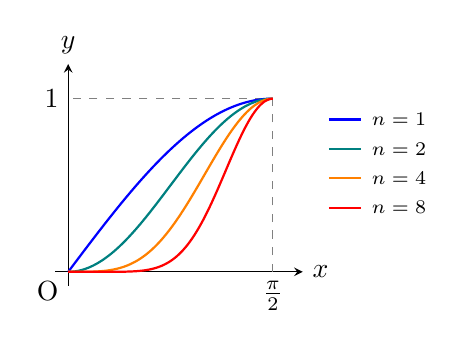
\begin{tikzpicture}[x=2.6cm/1.5708,y=2.2cm,>=stealth]
  \draw[->] (-0.1,0) -- (1.8,0) node[right] {$x$};
  \draw[->] (0,-0.08) -- (0,1.2) node[above] {$y$};
  \draw[dashed,gray] (1.5708,0) -- (1.5708,1) -- (0,1);
  \node[below] at (1.5708,0) {$\frac{\pi}{2}$};
  \node[left] at (0,1) {$1$};
  \node[below left] at (0,0) {O};
  \foreach \n/\c [count=\i] in {1/blue,2/teal,4/orange,8/red} {
    \draw[thick,\c,domain=0:1.5708,samples=60,smooth]
      plot (\x,{sin(\x r)^\n});
    % 凡例（グラフの右外）
    \draw[thick,\c] (2.0,{1.05-0.17*\i}) -- (2.25,{1.05-0.17*\i})
      node[right,black,font=\scriptsize] {$n=\n$};
  }
\end{tikzpicture}
\end{minipage}
\vspace{-1ex}
\[
  \frac{\pi}{2}
  = \lim_{m\to\infty}
    \frac{2\cdot 2\cdot 4\cdot 4\cdots 2m\cdot 2m}
         {1\cdot 3\cdot 3\cdot 5\cdots (2m-1)(2m+1)}
\]
\end{hosoku}

ちゃんと綺麗に\LaTeX で組版されることを確認するために，ビルドしてみてください。

\end{document}
